%h (here), le decimos que ponga la imagen m\'as o menos aqu\'i
%t (top), preferiblemente en la parte superior de la p\'agina
%b (bottom), preferiblemente en la parte inferior de la p\'agina
%p (page), que junte los objetos flotantes en una p\'agina
%! que ignore sus reglas internas de posicionamiento
%H que ponga la imagen justo aqu\'i, similar a h!
\begin{figure}[h]
\centering
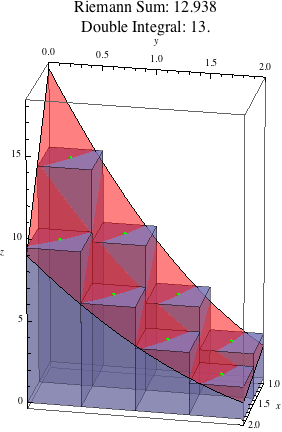
\includegraphics[width=5.5cm]{./extra/Riemann_double_integral.png}
\caption{Suma de Riemann en integrales dobles}
\label{fig:chaper01_01_Riemann_double_integral}
\end{figure}